\section{Introduction}\label{sec:hsamodel:introduction}

Continuum soft robots promise natural compliance and safe interaction with humans, thanks to their invertebrate-inspired bodies~\cite{della2020softencyclopedia}. Several actuation technologies for soft robots have been explored in recent years, with the most popular being cable-driven and pneumatic actuation~\cite{zaidi2021actuation}.
% Although pneumatically-driven soft robots have been successfully used~\cite{falkenhahn2015dynamic, franco2021position, zaidi2021actuation}, their speed is rather slow and their pneumatic actuation cannot generate twisting thus limiting their Degrees of Freedom (DoF) in task space.
% Cable-driven soft robots generate a pulling force with electric motors using a tendon attached to a soft structure, relying on the elasticity of the system to generate a motion.
%While similarly electrically actuated, 

\gls{HSA} robots are a recent development in this field~\cite{chin2018compliant, truby2021recipe, zhang2022vision}, which directly transform applied motor torques into complex motion primitives. % more citations: lipton2018handedness, chin2019automated
%
This novel type of actuator is based on an architected metamaterial. The most important characteristic of this cylindrical metamaterial is that twist strains along the handedness of the structure lead to an elongation of the rod, which is also called auxetic trajectory~\cite{good2022expanding}. 
% These twist strains can be imposed by electric actuation thus enabling fast system responses~\cite{garg2022kinematic}. 
An \gls{HSA} robot combines multiple \glspl{HSA} of different handedness with a platform constraining the movement of the distal ends in the fashion of a soft parallel manipulator. 
Differential elongation of the rods enables complex motion primitives such as elongation, bending, and twisting~\cite{chin2018compliant}, which can be seen in Fig.~\ref{fig:hsamodel:motion_primitives}. % lipton2018handedness
\gls{HSA} robots are particularly difficult to model and control as the forces and torques causing the evolution of the system are not directly produced by the actuator, but instead are intrinsically generated as an effect of the modified cell state of the metamaterial and of the interaction forces coming from the parallel arrangement.

\begin{figure}
    \centering
    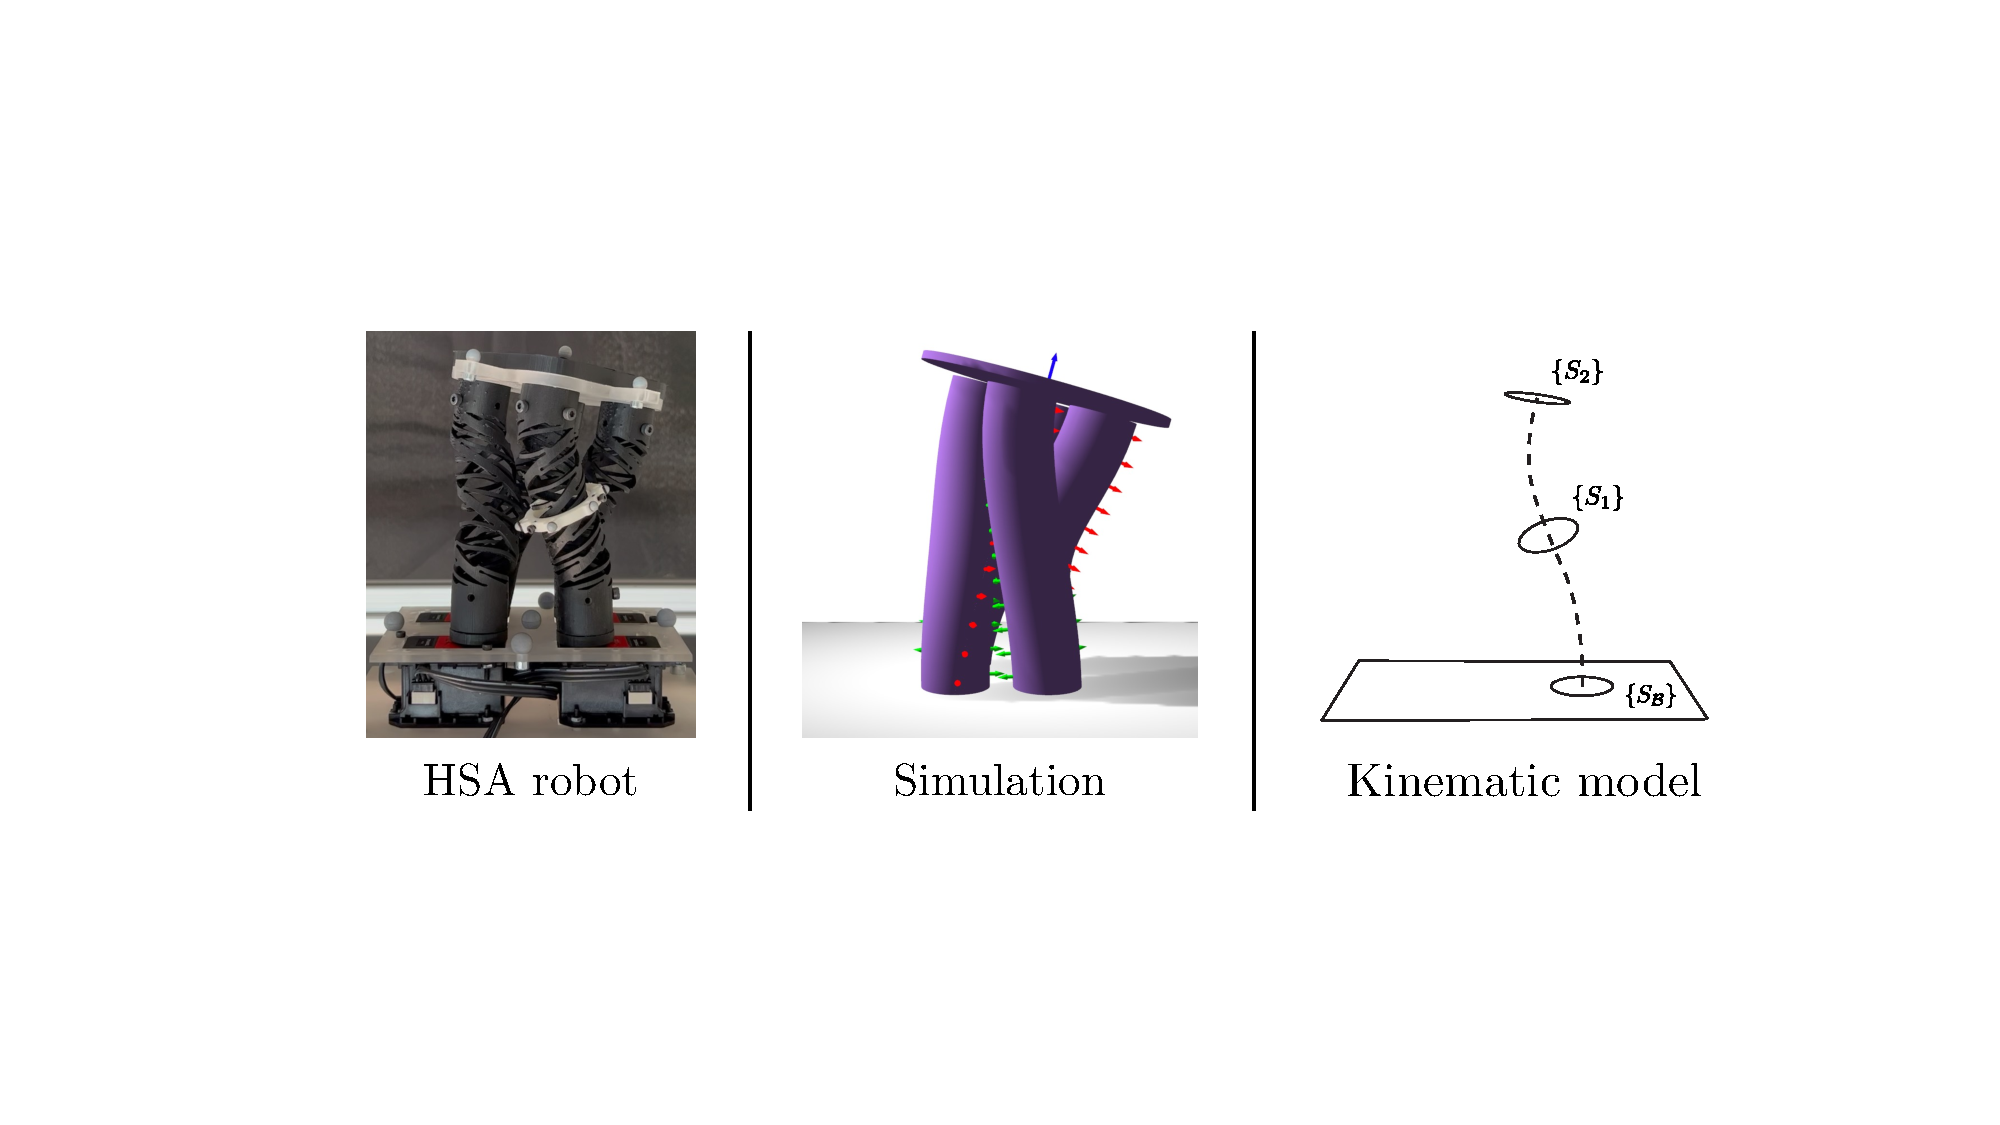
\includegraphics[width=0.72\columnwidth]{hsamodel/figures/overview/overview_v2_cropped.pdf}
    \caption{An HSA robot in a twisted state: simulation and schematic of kinematic model of single HSA rod.}
    \label{fig:hsamodel:overview}
\end{figure}

%This twist strain can be imposed by constraining the tip and simultaneously actuating the proximal end of the \glspl{HSA} with electric servo motors thus enabling fast system responses~\cite{garg2022kinematic}. Combining multiple rods (usually four) of different handedness with a platform at the distal end creates a \gls{HSA} robot. Differential elongation of the rods and leveraging the torsional torques by the motors enable complex motion primitives such as elongation, bending, and twisting~\cite{chin2018compliant, lipton2018handedness}, which can be seen in Fig.~\ref{fig:hsamodel:motion_primitives}.

% This novel type of soft robot consists of four pillars of architected metamaterials.
% The important characteristic of each of the cylindrical auxetics is that twist strains following the handedness of the pattern cause an elongation of the rod. 
% Each of these \glspl{HSA} is independently actuated using electric servo motors thus enabling fast system responses~\cite{garg2022kinematic}.

% Although the latest advances in 3D-printing of metamaterials via digital projection lithography~\cite{truby2021recipe} have made the manufacturing of \gls{HSA} robots much easier, the technology is still expensive and in its infancy. This lack of accessibility severely limits the progress on modelling the behaviour of \gls{HSA} robots and control them successfully. Therefore, a fast simulator is a necessity to allow the research community to rapidly prototype new control strategies.
\gls{FEM} based approaches~\cite{farrell2020extension} have proven to be effective in simulating soft parallel structures \cite{vanneste2021enabling} and could be a good candidate for representing the complex behavior of \gls{HSA} robots. However, in this paper we strive for a less computationally expensive solution - towards applications in model based control \cite{della2023model}. For this reason, we look at the framework of the \gls{DCM}. The Cosserat rod theory assumes the slenderness of the object, e.g. that the length is much larger than the radius, and allows for the rod to exhibit all six principal strains. The 1D discretization of the rod along its length dramatically reduces the computational demand compared to \gls{FEM}~\cite{gazzola2018forward}. 
% The main modification compared to the SoA simulators~\cite{naughton2021elastica, mathew2022sorosim} is that we couple the twist strains to the rest length of the rod. 
%
Several works in recent literature have successfully applied this framework to soft robotics \cite{grazioso2019geometrically,sadati2021tmtdyn,armanini2021soft}. Among them, in \gls{PCS}~\cite{renda2018discrete} the continuum dynamics of the Cosserat model is discretized in space by keeping a selection of strains constant along a segment of the continuum. %They all neglect volumetric deformations and focus on the behaviour of the central axis~\cite{della2021model}. 
The most popular \gls{PCS} is \gls{PCC}~\cite{webster2010design}, which assumes a sequence of arcs. Functional extensions of \gls{PCS} use continuous function to approximate the strain~\cite{della2019control,renda2020geometric}. %The functional subspace is split into basis functions and weights, which are taken as the configuration of the robot~\cite{della2021model}. 
% Finally, \gls{FEM} models represent the shape of the continuum with a mesh~\cite{grazioso2019geometrically}, therefore not neglecting the volumetric deformations.

However, none of these methods are currently applicable to HSA robots, as they do not embed a mechanism for incorporating the effect of the auxetic trajectory.
%
We are aware of just one work looking into kinematic modeling of HSA robots~\cite{garg2022kinematic}, which however models the backbone of the robot with \gls{PCC} instead of modeling the HSAs. As a consequence, the model cannot represent complex behaviors of the module, like the twist in Fig.~\ref{fig:hsamodel:overview}. 

The goal of this paper is to provide such a mechanism, to introduce a strategy for further reducing the dimensionality of the model, and to provide extensive experimental validation to both. More specifically, our extension to the \gls{DCM} framework couples the twist strain of the \gls{HSA} rod to its rest length. %The elastic modulus together with the axial strains will then naturally drive the \gls{HSA} towards this rest length.
Additionally, we allow the rigidity of the rod to be modified as a function of the twist strain. %This is necessary as new work on identifying the mechanical characteristics of \glspl{HSA}~\cite{good2022expanding} has shown that the spring constant increases with the twist strains.
We have implemented this mechanism as a plugin for Elastica~\cite{naughton2021elastica}, which we provide open source~\footnote{\scriptsize \url{https://github.com/tud-phi/HSA-PyElastica}}. 
This results in a compact dynamic model that we test experimentally.
% Several SoA simulators simulators~\cite{naughton2021elastica, mathew2022sorosim} rely on this discretized Cosserat rod theory. 

\begin{figure*}[hbt]
    \centering
    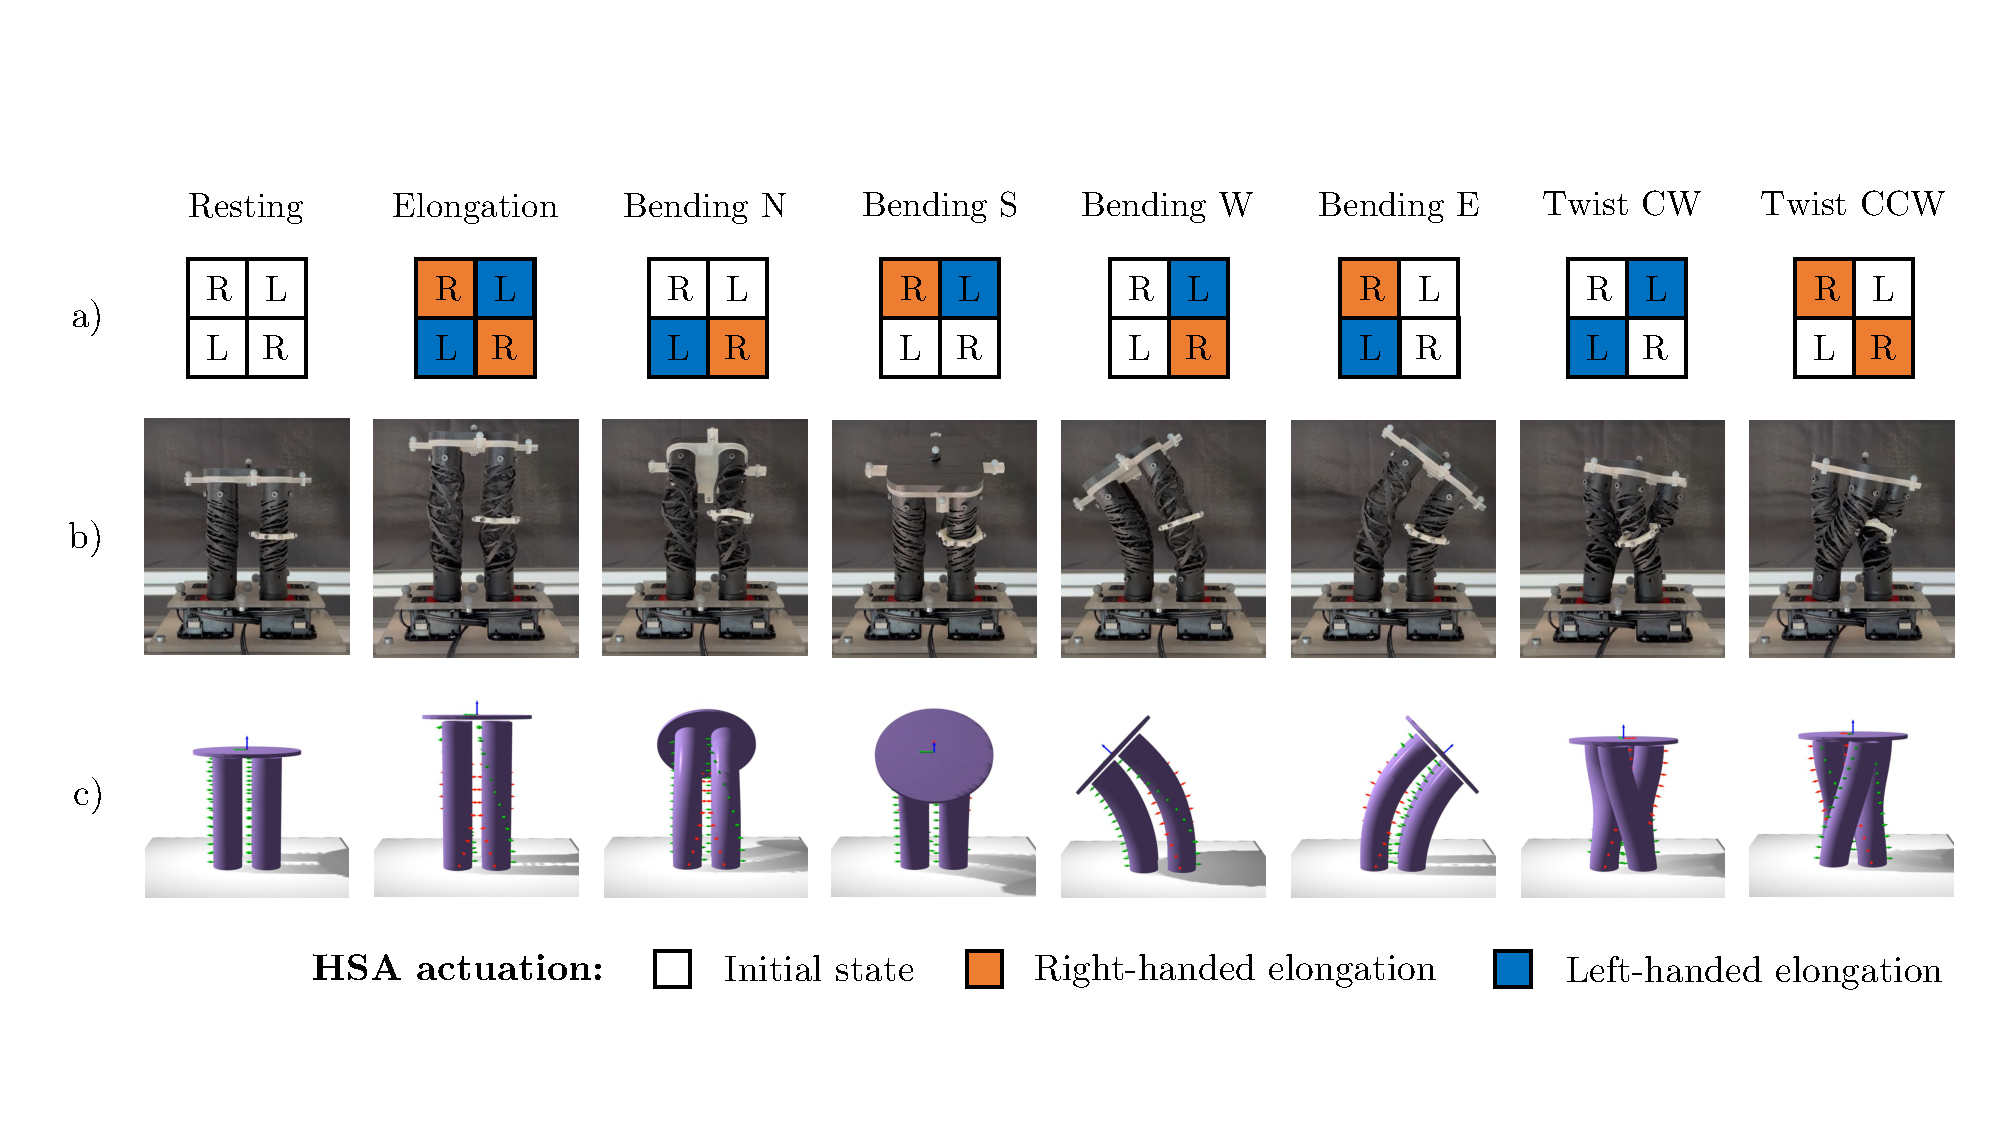
\includegraphics[width=1.0\textwidth]{hsamodel/figures/motion_primitives/motion_primitives_v2_compressed.pdf}
    
    \caption{Motion primitives of Handed Shearing Auxetic (HSA) robots: elongation, bending in the four cardinal directions (e.g. north (N), south (S), west (W), east (E)), and clock-wise (CW) and counter-clockwise (CCW) twisting.
    \textbf{First row (a):} depicts the necessary actuation inputs to generate these motion primitives. Pure elongation is achieved by applying the motor torques of the same magnitude but opposite direction to the left-handed (L) and right-handed (R) HSAs. For bending, there exists a delta in elongation of the rods while the sum of torques is still zero. Last but not least, counter-clockwise twisting is achieved by applying more torque to the right-handed, than to the left-handed HSA rods.
    \textbf{Second row (b):} Snapshots of the experimental platform when actuated according the above specified sequence.
    \textbf{Third row (c):} Renderings of simulated steady-states of an HSA robot. It consists of four HSA rods and a platform at the distal end. The red arrows point along the local x-axis and the green arrows along the local y-axis respectively. The blue arrow signifies the z-axis of the local frame of the platform.}\label{fig:hsamodel:motion_primitives}
\end{figure*}

%To move towards effective model-based control approaches with a manageable computational demand and sensing requirements, 
% For control purposes, we strive for low-dimensional kinematic parametrizations of the configuration of the system~\cite{della2021model}. 
%Namely, kinematic models provide us with a finite-dimensional approximation of the integral system behavior and are the integral foundation of model-based controllers~\cite{della2021model}
% Namely, kinematic models provide us with Cartesian-space pose information for a given configuration of the robot.
%
%
%

%
We then use a combination of \gls{CS} and \glspl{PCS}~\cite{renda2018discrete} to describe the shape of \gls{HSA} rods, which we call a \gls{SPCS} model: while some strains, such as twist \& stretch, are mostly constant over the length of the entire \gls{HSA}, other strains such as bend \& shear significantly vary and are thus captured in a piecewise parametrization. We provide an open-source implementation of this kinematic model in JAX~\footnote{\scriptsize \url{https://github.com/tud-phi/jax-spcs-kinematics}}.

% Our results show that a kinematic parametrization with $11$ Degrees of Freedom (DoF) is sufficient to capture the shape of \glspl{HSA}. The parametrization keeps the twist \& stretch constant across the entire length of the rod and uses two \gls{PCS} segments to represent the bend \& shear deformations.
% Compared to the Cosserat rod model used for simulating \glspl{HSA}, we have therefore significantly reduced the DoF of the kinematics.

In summary, we contribute to the state of the art in modeling of soft robots with:
%
\begin{enumerate}
    \item A mechanism for integrating the auxetic trajectory of \glspl{HSA} into the discrete Cosserat rod theory~\cite{gazzola2018forward, mathew2022sorosim}. %Specifically, we modify the rest length of the rod as a function of the twist strain to cause an elongation of the \gls{HSA}.
    \item A plugin for the Elastica simulator~\cite{naughton2021elastica}, which also includes the necessary boundary conditions and joint formulations to simulate \gls{HSA} robots.
    \item A Selective Piecewise Constant Strain (SPCS) kinematic model to parameterize the shape of \glspl{HSA} with a dramatically reduced number of states. %Namely, we combine strain components constant along the entire length with piece-wise constant strains. %This concept allows us to dramatically reduce the dimensionality of the model, which is ideal for control purposes. We verify this model's ability to describe the shape of the rods of an \gls{HSA} robot in both simulation and experimentally.
\end{enumerate}
% \begin{itemize}
%     \item We infuse the auxetic trajectory into the discretized Cosserat rod theory to build a dynamical simulator of HSA robots and add support for the common mechanical characteristics of \gls{HSA} rods.
%     \item We show that the shape of \gls{HSA} rods can be kinematically described by very few parameters within the \gls{PCS} framework. This twist-aware kinematic model is able to reconstruct the local orientation of the \gls{HSA} rods and is with that also suitable for twisting motion primitives.
%     % \item We propose a kinematic parametrization for \gls{HSA} rods, which are i) able to derive the local orientation of the rod, and ii) also are suitable for the twisting motion primitive of \gls{HSA} robots.
% \end{itemize}
Contributions (1) and (2) are covered in Section~\ref{sec:hsamodel:simulation}. Subsequently, we introduce the kinematic model from contribution (3) in Section~\ref{sec:hsamodel:kinematic_model} and verify it in Section~\ref{sec:hsamodel:verification_kinematics}.